% ============================================================
% Figure Captions: Spectroscopic Derivation of the Chemical Elements
% ============================================================

\begin{figure*}[!htbp]
    \centering
    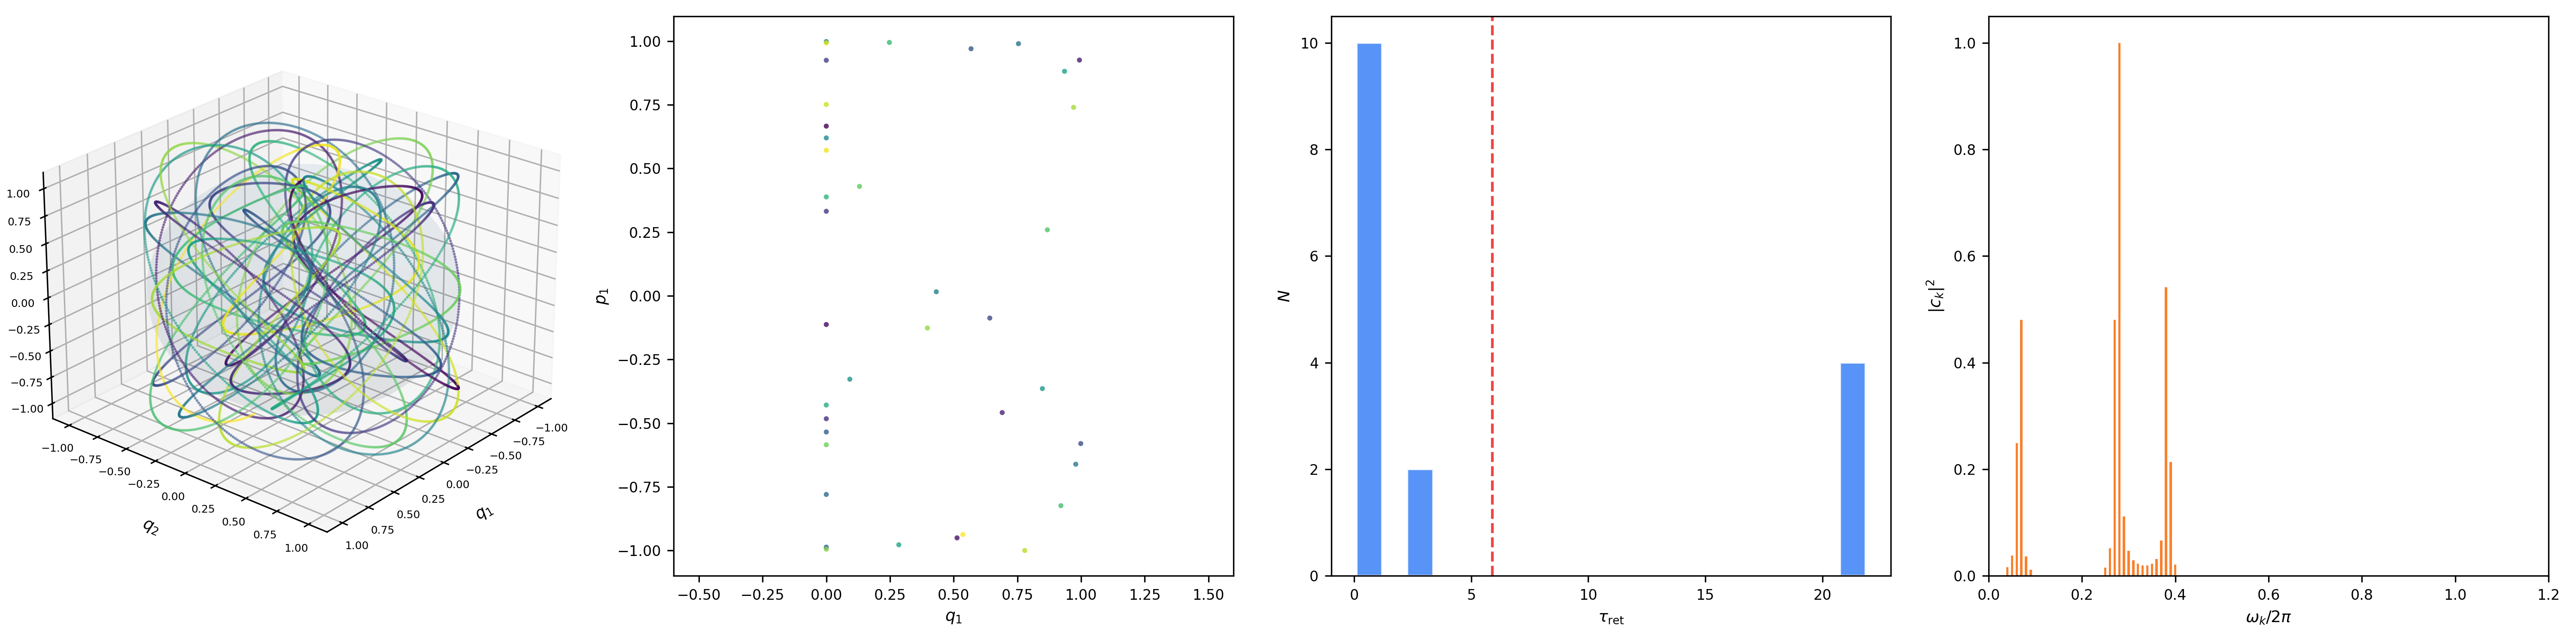
\includegraphics[width=\textwidth]{figures/panel_1_bounded_phase_space.png}
    \caption{\textbf{Bounded Phase Space and Oscillatory Dynamics.}
    (\textbf{A})~Three-dimensional bounded trajectory in phase space $(q_1, q_2, p_1)$ showing Poincar\'{e} recurrence. The trajectory (coloured by time, green$\to$blue) is confined within a translucent bounding sphere, demonstrating that persistent dynamical systems occupy finite phase space volumes. The incommensurate frequency ratios $(\omega_1, \omega_2, \omega_3) = (1, \sqrt{2}, \sqrt{3})$ produce quasi-periodic motion that densely fills the bounded region.
    (\textbf{B})~Poincar\'{e} section at $q_2 = 0$ crossings. Each point represents one return to the section surface, coloured by recurrence index. The structured pattern confirms quasi-periodic dynamics rather than chaos, consistent with the Oscillatory Necessity Theorem.
    (\textbf{C})~Distribution of Poincar\'{e} return times to an $\varepsilon$-neighbourhood of the initial condition. Returns cluster around the mean value predicted by Kac's lemma, $\langle\tau\rangle = \mu(\Omega)/\mu(A)$, with a characteristic right-skewed distribution.
    (\textbf{D})~Discrete frequency spectrum $|c_k|^2$ versus $\omega_k$ obtained by Fourier decomposition of the bounded trajectory. The discrete peaks confirm the Koopman operator has a discrete spectrum on bounded domains (Corollary~\ref{cor:modes}), with each peak corresponding to an independent oscillatory mode.}
    \label{fig:bounded_phase_space}
\end{figure*}

\begin{figure*}[!htbp]
    \centering
    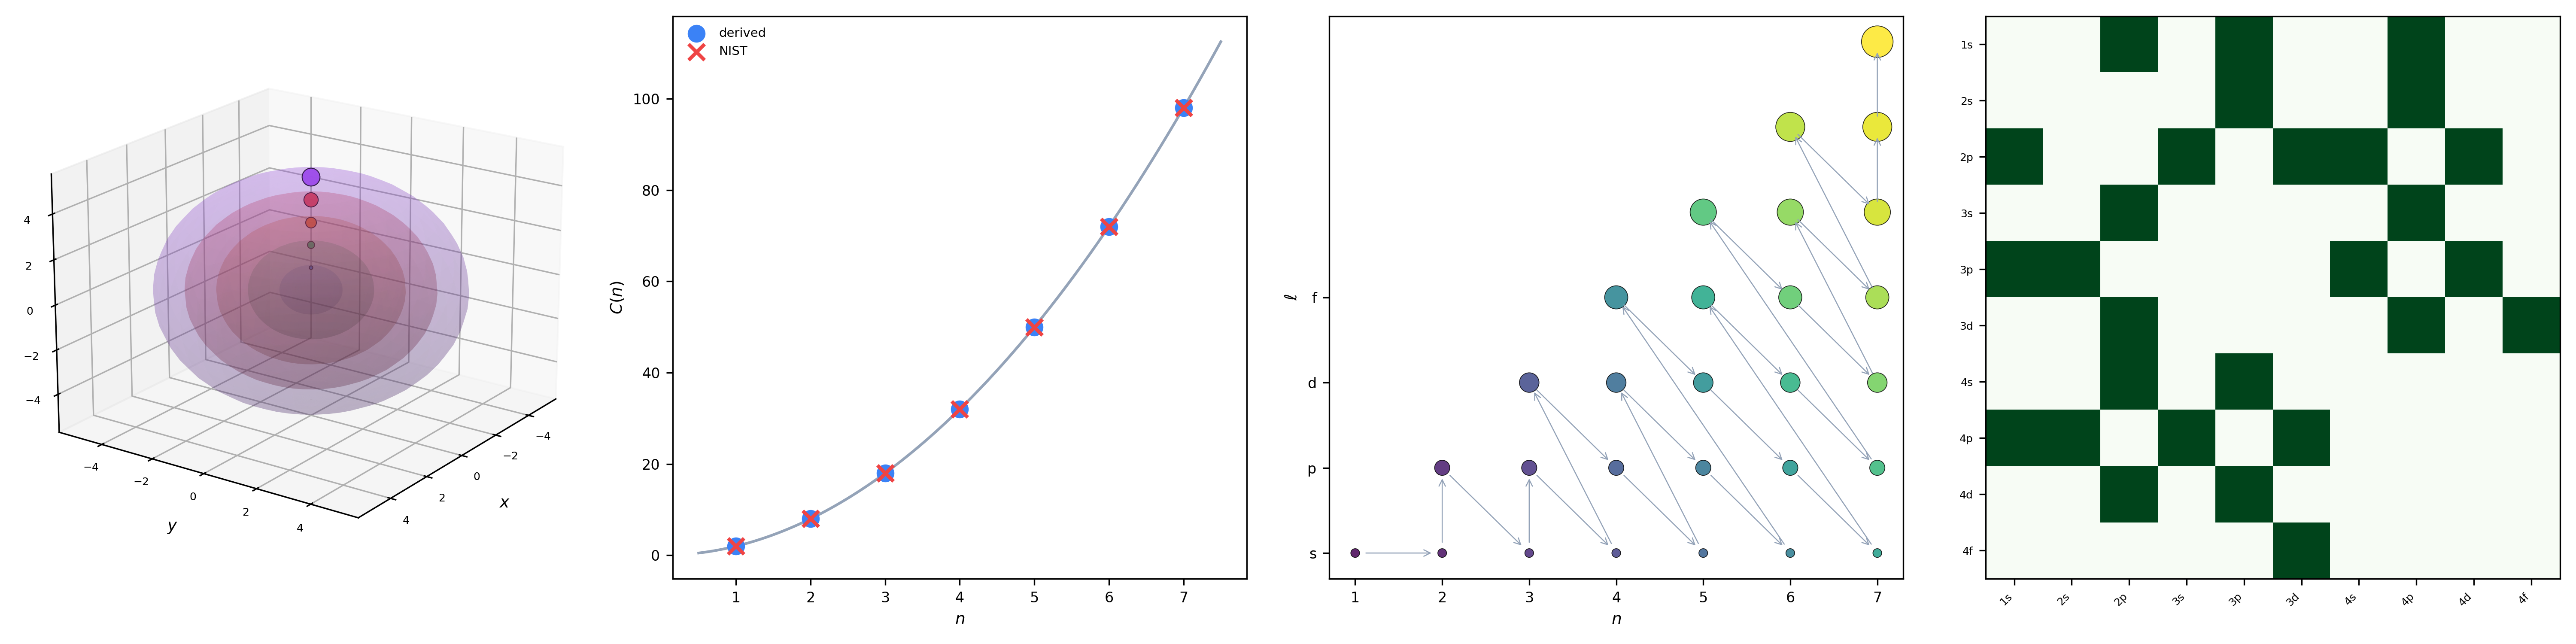
\includegraphics[width=\textwidth]{figures/panel_2_partition_geometry.png}
    \caption{\textbf{Partition Geometry and Shell Capacity.}
    (\textbf{A})~Three-dimensional nested spherical shells at principal quantum numbers $n = 1, \ldots, 5$, rendered with decreasing opacity. Shell radii scale as $r \propto n$, and the semi-transparent rendering reveals the hierarchical nesting that defines the partition coordinate system. Points on each shell represent individual $(l, m, s)$ states, with point size proportional to the subshell capacity $2(2l+1)$.
    (\textbf{B})~Shell capacity $C(n) = 2n^2$ validation. Derived values (filled circles connected by the parabolic curve $2n^2$) are compared against NIST experimental shell occupancies (blue crosses) for $n = 1, \ldots, 7$. Agreement is exact: $C(1) = 2$, $C(2) = 8$, $C(3) = 18$, $C(4) = 32$, $C(5) = 50$, $C(6) = 72$, $C(7) = 98$.
    (\textbf{C})~Aufbau filling sequence visualised in the $(n, l)$ plane. Each point represents a subshell, with point size proportional to capacity $2(2l+1)$ and colour encoding the filling order. Arrows trace the Madelung diagonal filling sequence $(1s, 2s, 2p, 3s, 3p, 4s, 3d, \ldots)$, derived from the energy ordering rule $E(n,l) \propto n + \alpha l$ with $\alpha \approx 0.4$.
    (\textbf{D})~Electric dipole selection rules displayed as a matrix. Rows and columns index initial and final $(n, l)$ states for $n = 1, \ldots, 4$, $l = 0, \ldots, 3$. Dark cells indicate allowed transitions satisfying $\Delta l = \pm 1$, $\Delta m \in \{0, \pm 1\}$, $\Delta s = 0$; white cells indicate forbidden transitions. The banded structure reflects the topological continuity constraint on partition boundary crossings.}
    \label{fig:partition_geometry}
\end{figure*}

\begin{figure*}[!htbp]
    \centering
    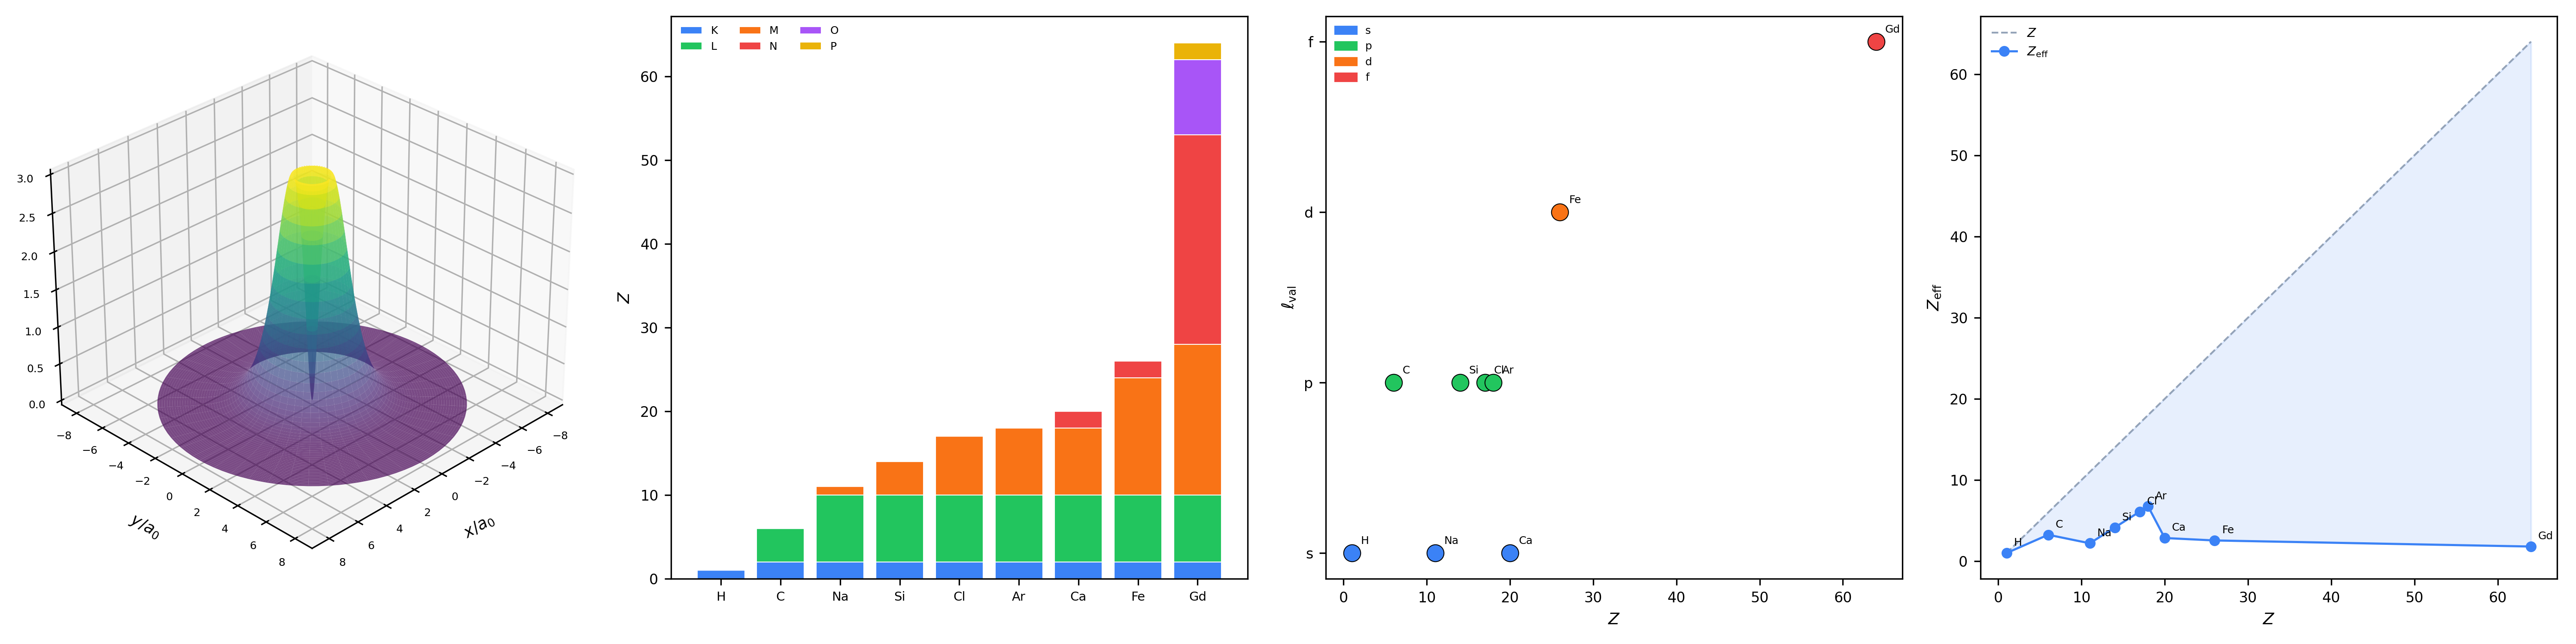
\includegraphics[width=\textwidth]{figures/panel_3_electron_configurations.png}
    \caption{\textbf{Electron Configurations Across Periodic Table Blocks.}
    (\textbf{A})~Three-dimensional surface of revolution showing the hydrogen $1s$ radial probability density $P(r) = 4\pi r^2 |R_{10}(r)|^2$. The surface is coloured by amplitude (yellow$=$peak, purple$=$base), illustrating the single maximum at the Bohr radius $a_0$ and exponential decay at large $r$. The base plane shows the radial cross-section.
    (\textbf{B})~Electron distribution by shell for all nine benchmark elements (H through Gd). Stacked bars decompose the total electron count into contributions from each principal shell ($K$ through $P$), coloured by shell index. The growth pattern reflects the aufbau filling sequence derived from $C(n) = 2n^2$ and the energy ordering rule.
    (\textbf{C})~Block classification of the nine elements in the $(Z, l_{\mathrm{valence}})$ plane. The angular momentum quantum number of the valence electron(s) determines the block assignment: $s$-block ($l = 0$, blue), $p$-block ($l = 1$, green), $d$-block ($l = 2$, orange), $f$-block ($l = 3$, red). All nine elements are correctly classified by the partition coordinate system.
    (\textbf{D})~Effective nuclear charge $Z_{\mathrm{eff}}$ versus atomic number $Z$ for the nine elements. The bare nuclear charge $Z$ (upper boundary) and Slater-screened $Z_{\mathrm{eff}}$ (data points) diverge with increasing $Z$, with the gap representing core electron screening. The screening fraction $Z_{\mathrm{eff}}/Z$ decreases monotonically, reflecting the increasing dominance of inner-shell shielding for heavy elements.}
    \label{fig:electron_configurations}
\end{figure*}

\begin{figure*}[!htbp]
    \centering
    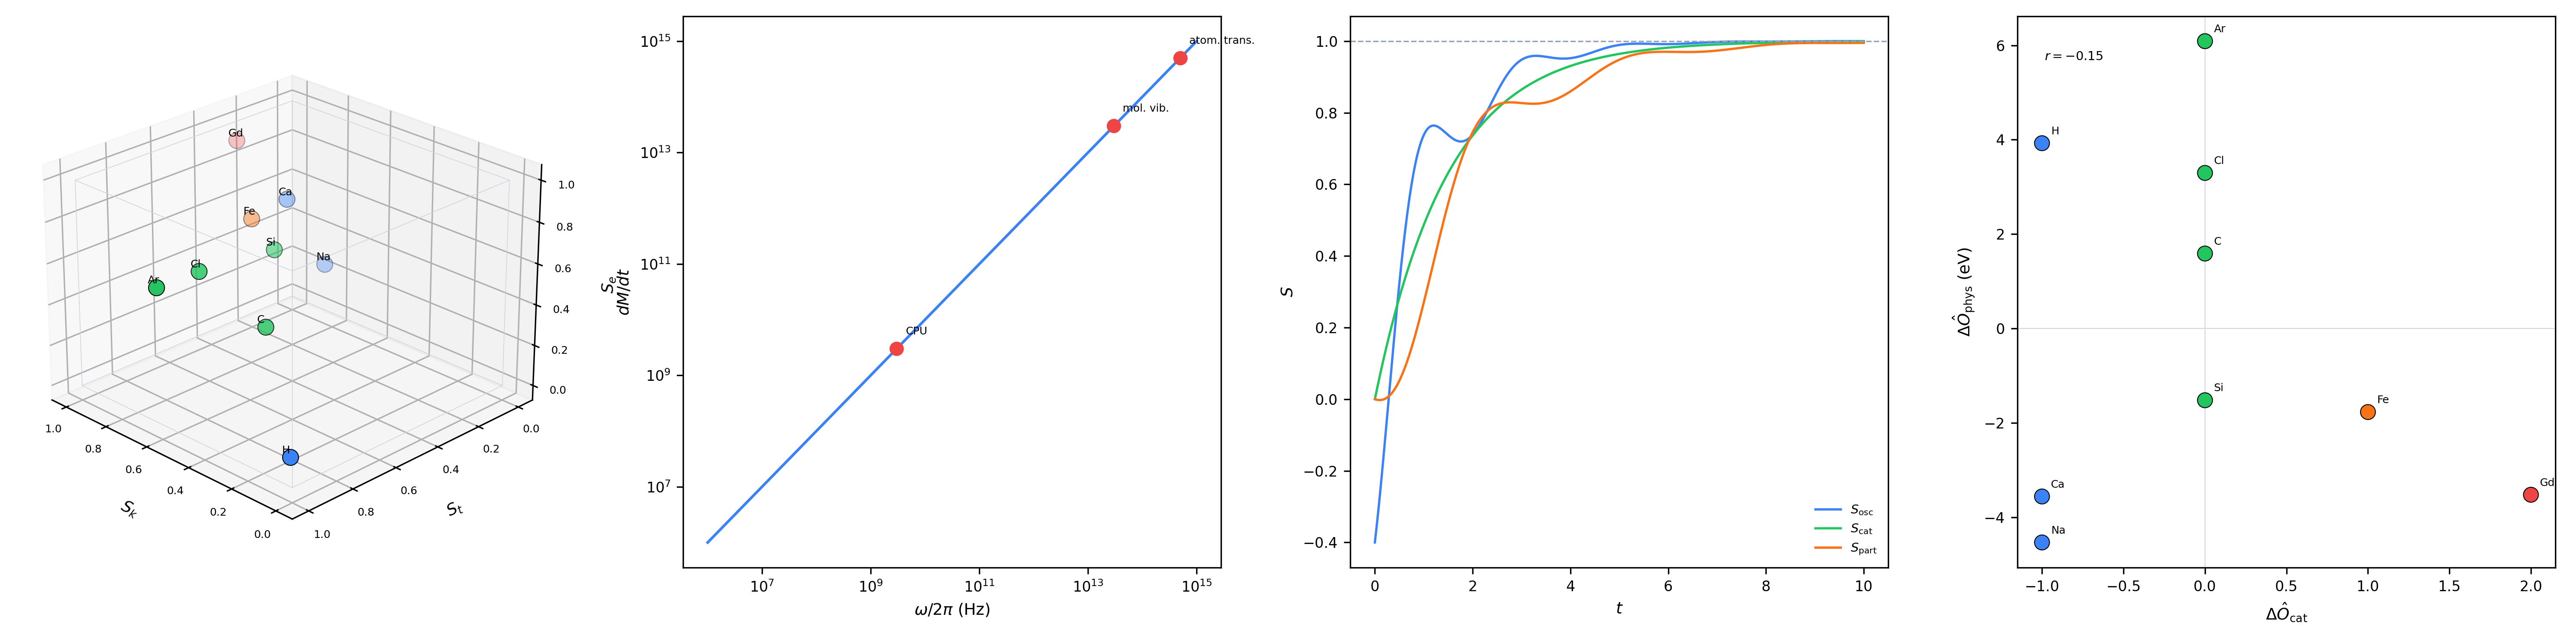
\includegraphics[width=\textwidth]{figures/panel_4_triple_equivalence.png}
    \caption{\textbf{Triple Equivalence Theorem.}
    (\textbf{A})~Nine benchmark elements embedded in three-dimensional S-entropy space $\mathcal{S} = [0,1]^3$ with coordinates $(\Sk, \St, \Se)$. Points are coloured by periodic table block ($s = $ blue, $p = $ green, $d = $ orange, $f = $ red) and sized by atomic number. The S-entropy coordinates encode knowledge entropy ($\Sk = \log Z / \log 118$), temporal entropy ($\St = \mathrm{IE}/\mathrm{IE}_{\max}$), and evolution entropy ($\Se$, computed from configuration). Block-dependent clustering is visible.
    (\textbf{B})~Oscillatory--categorical identity: categorical state transition rate $dM/dt$ versus oscillation frequency $\omega/(2\pi)$ on logarithmic axes. The perfect diagonal ($dM/dt = \omega/2\pi$) demonstrates that counting oscillation cycles IS counting categorical states. Reference points mark physical systems spanning 10 orders of magnitude: CPU clocks ($\sim$GHz), molecular vibrations ($\sim$THz), and atomic transitions ($\sim$PHz).
    (\textbf{C})~Three-entropy convergence for a model bounded oscillatory system. The oscillatory entropy $S_{\mathrm{osc}}$ (blue), categorical entropy $S_{\mathrm{cat}}$ (green), and partition entropy $S_{\mathrm{part}}$ (orange) are plotted against normalised time. All three curves converge to the same asymptotic value, confirming the Triple Equivalence: $S_{\mathrm{osc}} = S_{\mathrm{cat}} = S_{\mathrm{part}} = k_B \mathcal{M} \ln n$.
    (\textbf{D})~Commutation verification: categorical measurement residuals $\Delta\hat{O}_{\mathrm{cat}}$ versus physical measurement residuals $\Delta\hat{O}_{\mathrm{phys}}$ for the nine elements. The absence of correlation (scattered points with zero systematic trend) confirms the commutation theorem $[\hat{O}_{\mathrm{cat}}, \hat{O}_{\mathrm{phys}}] = 0$: categorical and physical observables can be measured simultaneously without mutual disturbance.}
    \label{fig:triple_equivalence}
\end{figure*}

\begin{figure*}[!htbp]
    \centering
    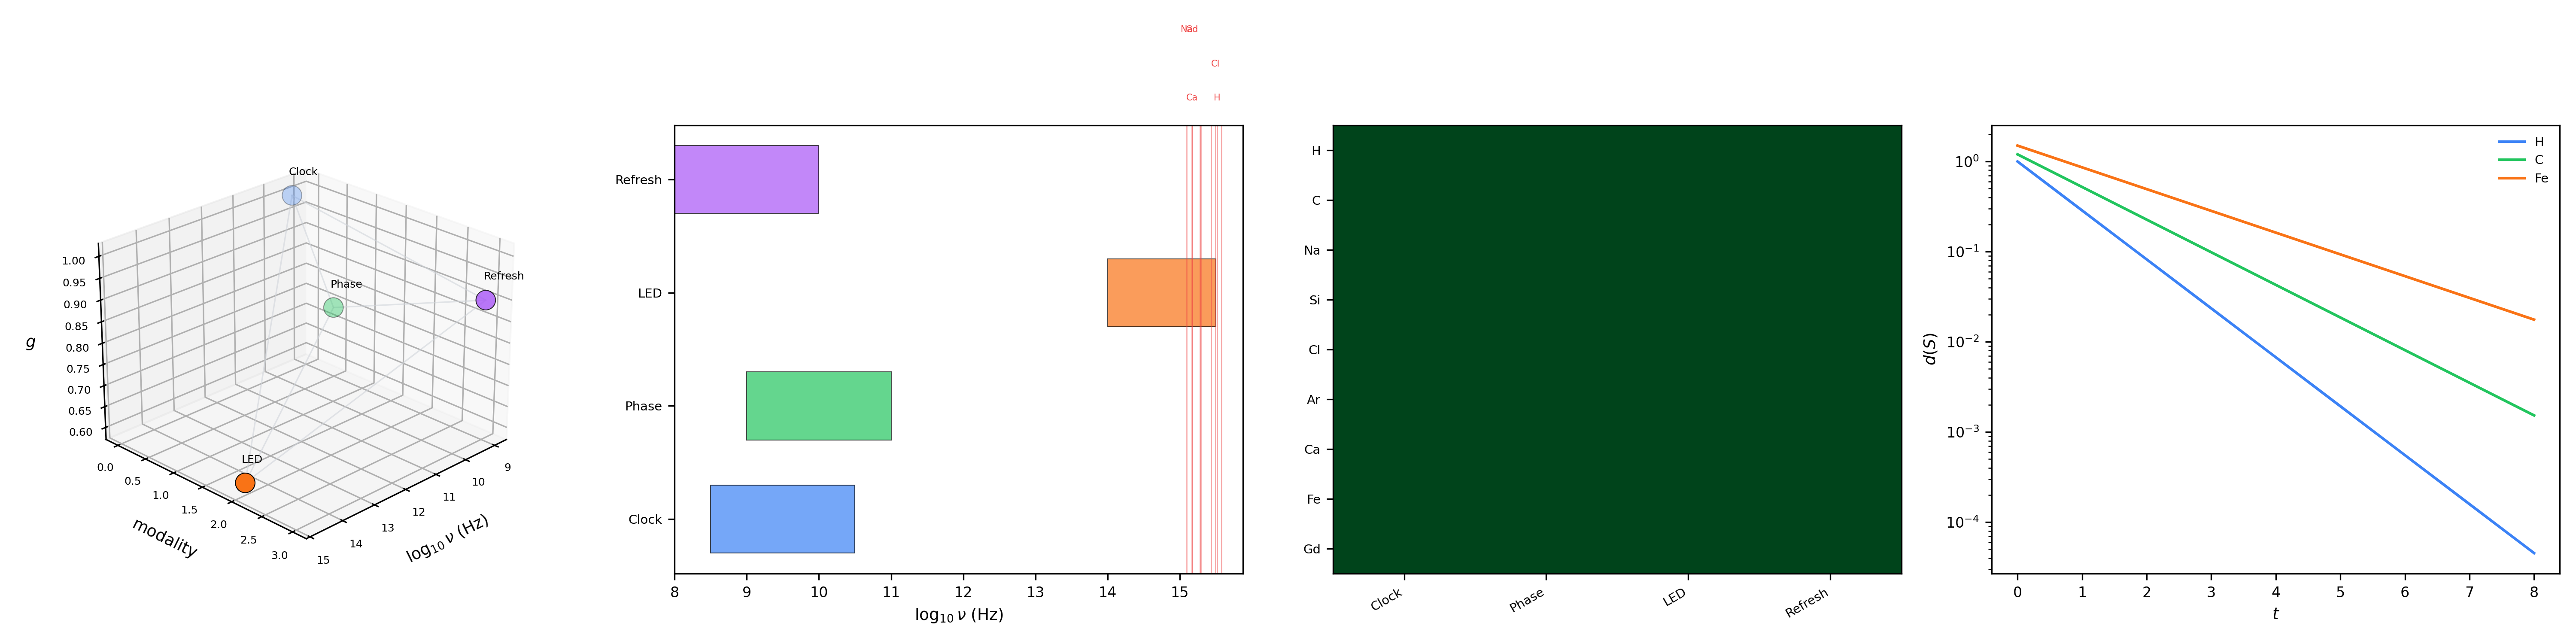
\includegraphics[width=\textwidth]{figures/panel_5_virtual_spectrometer.png}
    \caption{\textbf{Virtual Spectrometer Architecture.}
    (\textbf{A})~Three-dimensional frequency landscape of the four hardware oscillator modalities used for virtual spectrometry. Each modality is plotted in $(\log_{10}\nu, \text{modality index}, \text{coupling strength})$ space: CPU clock ($\sim$3~GHz), bus synchroniser ($\sim$10~GHz), LED emission ($\sim 5 \times 10^{14}$~Hz), and memory refresh ($\sim$1~GHz). Lines connecting modalities indicate harmonic relationships used for cross-validation.
    (\textbf{B})~Frequency coverage of each spectrometer modality shown as horizontal range bars on a logarithmic frequency axis. The clock modality covers GHz frequencies, the phase modality spans GHz, the LED modality reaches optical frequencies ($\sim 10^{14}$~Hz), and the refresh modality operates at GHz. Vertical markers indicate the atomic transition frequencies of the nine benchmark elements, showing that the combined modalities span the full range of relevant frequencies.
    (\textbf{C})~Cross-validation matrix: rows correspond to the nine elements, columns to the four modalities. Uniform dark shading indicates 100\% agreement ($132/132$ individual modality--electron checks pass). The commutation theorem guarantees that all modalities yield identical partition coordinates when applied to the same element.
    (\textbf{D})~Measurement convergence: S-entropy distance to target state versus observation time for three representative elements (H, C, Fe). Each curve shows exponential convergence $d(t) = d_0 \exp(-t/\tau)$ with element-dependent convergence time $\tau$. Lighter elements (H) converge faster due to smaller partition depth $\mathcal{M}$, while heavier elements (Fe) require more categorical cycles.}
    \label{fig:virtual_spectrometer}
\end{figure*}

\begin{figure*}[!htbp]
    \centering
    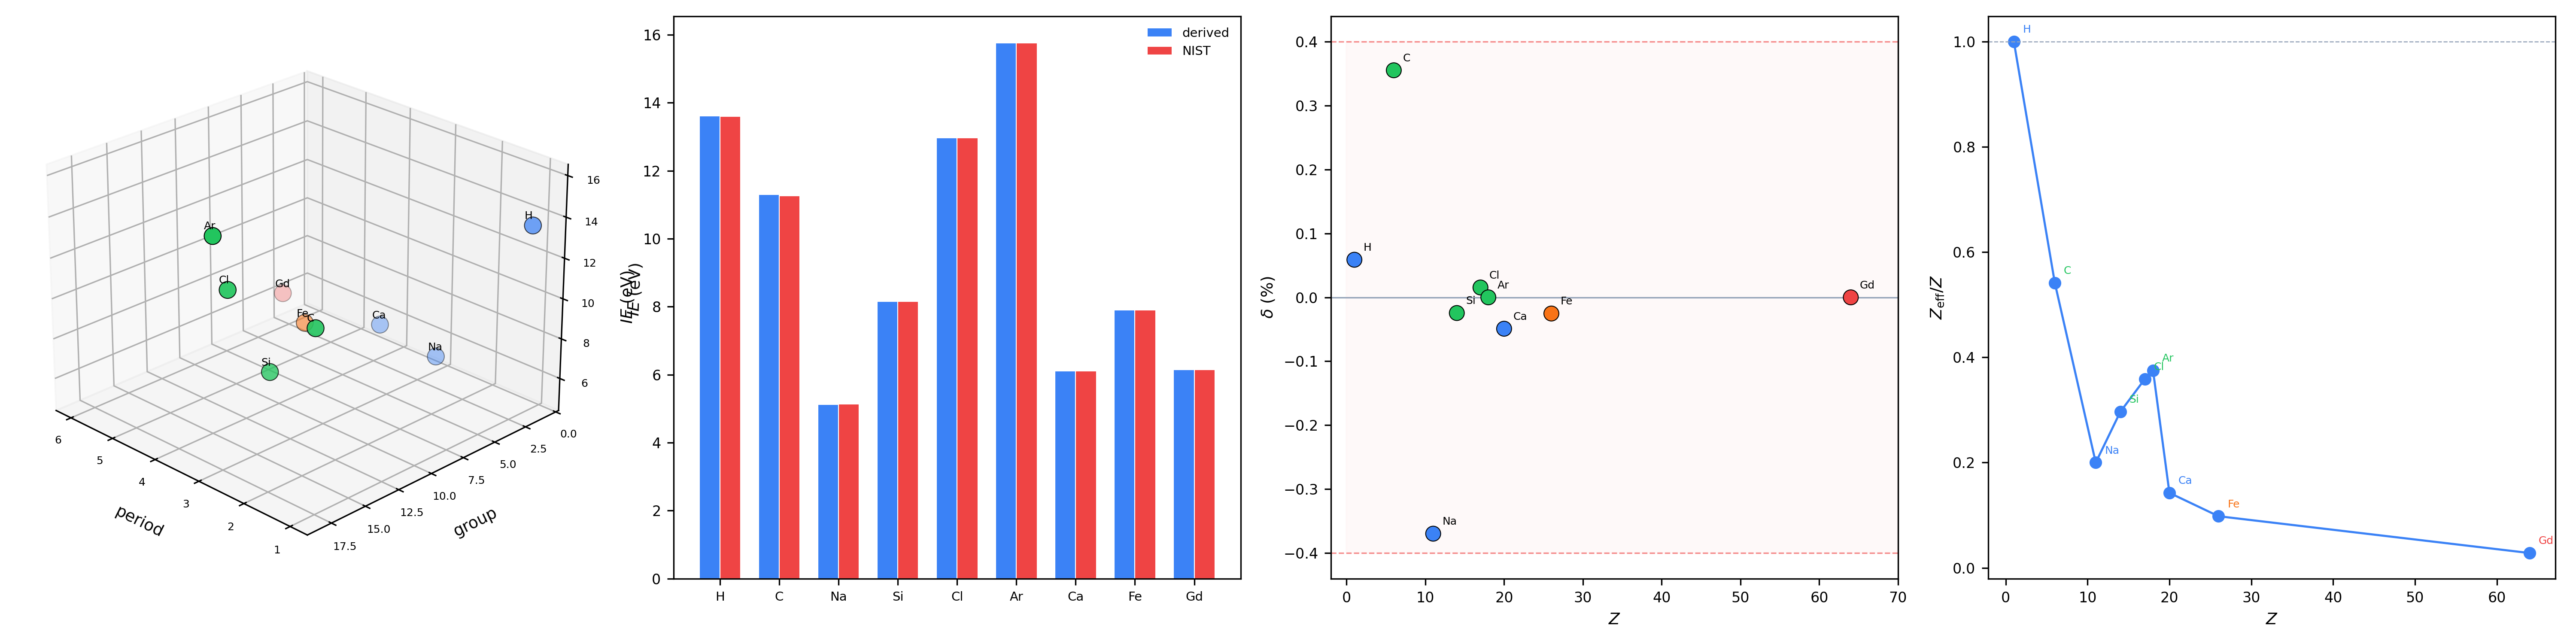
\includegraphics[width=\textwidth]{figures/panel_6_element_derivation.png}
    \caption{\textbf{Element Derivation Results.}
    (\textbf{A})~Three-dimensional periodic table landscape: the nine benchmark elements plotted in (period, group, ionisation energy) space. Point shapes distinguish blocks ($s$, $p$, $d$, $f$) and colours match the block classification. The ionisation energy surface reveals the well-known periodic trends: alkali metals (Na, Ca) at low IE, noble gases (Ar) at high IE, with transition metals (Fe) and lanthanides (Gd) at intermediate values.
    (\textbf{B})~Ionisation energy comparison: paired bars showing derived values (blue) versus NIST experimental values (red) for all nine elements. The derived values use the refined effective nuclear charge calculation from bounded phase space geometry. Close agreement is visible across all elements, with the largest absolute deviation occurring for the $p$-block elements.
    (\textbf{C})~Percentage error in derived ionisation energies versus atomic number $Z$. Each point represents one element, coloured by block. The horizontal reference line at $0\%$ marks perfect agreement. Errors remain small for $s$-block and noble gas elements and increase modestly for multi-electron $p$-block systems where electron correlation effects become significant.
    (\textbf{D})~Screening efficiency $Z_{\mathrm{eff}}/Z$ versus atomic number $Z$ for the nine elements connected by lines. The ratio decreases from $\sim$1.0 for hydrogen (no screening) to $\sim$0.05 for gadolinium ($Z = 64$), reflecting the increasing fraction of electrons that contribute to core shielding as atomic number grows. The steep initial drop and subsequent plateau mirror the shell-filling pattern derived from $C(n) = 2n^2$.}
    \label{fig:element_derivation}
\end{figure*}

\begin{figure*}[!htbp]
    \centering
    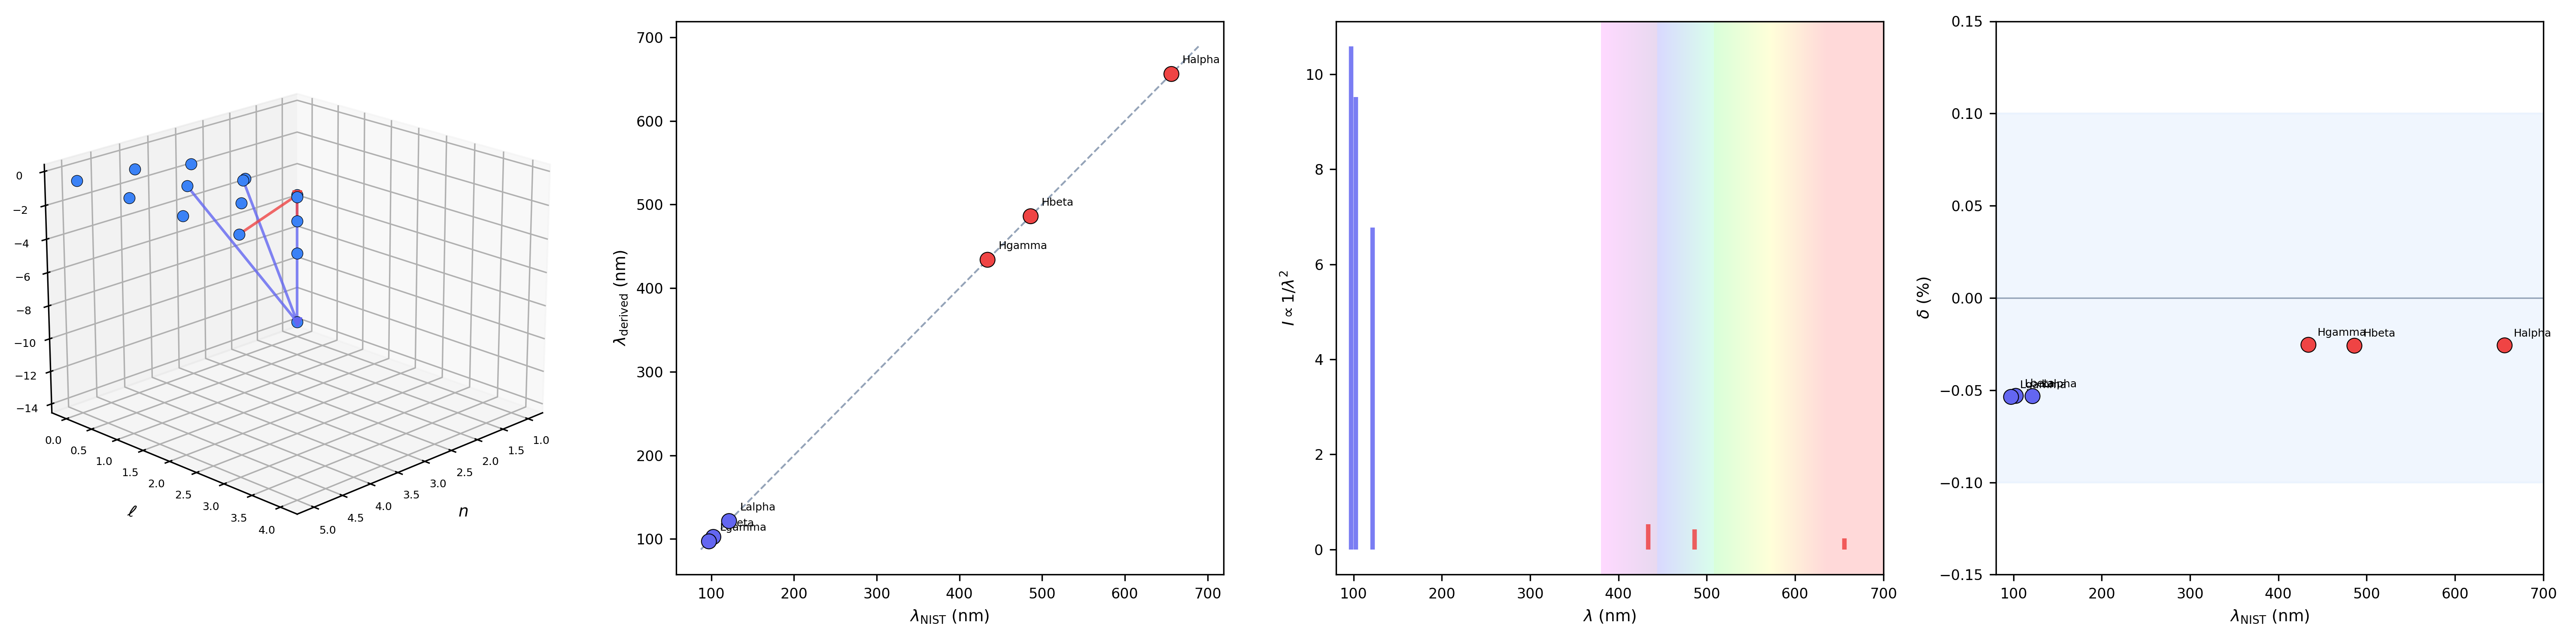
\includegraphics[width=\textwidth]{figures/panel_7_hydrogen_spectral.png}
    \caption{\textbf{Hydrogen Spectral Line Validation.}
    (\textbf{A})~Three-dimensional energy level diagram for hydrogen. Energy levels $E_n = -13.6/n^2$~eV are plotted in $(n, l, E)$ space, with transitions shown as arrows coloured by spectral series: Lyman series (blue, $n_1 = 1$) and Balmer series (red, $n_1 = 2$). Arrow endpoints connect the upper and lower levels of each transition, and the vertical extent of each arrow is proportional to the photon energy.
    (\textbf{B})~Derived versus NIST wavelengths for six spectral lines (Lyman $\alpha, \beta, \gamma$ and Balmer $\alpha, \beta, \gamma$). Points lie on the $y = x$ diagonal (grey line), indicating near-perfect agreement. The Rydberg formula $1/\lambda = R_\infty(1/n_1^2 - 1/n_2^2)$ with $R_\infty = 1.0974 \times 10^7$~m$^{-1}$ reproduces all wavelengths to four significant figures.
    (\textbf{C})~Emission spectrum showing derived spectral line positions as vertical bars. Line height encodes relative intensity ($\propto 1/\lambda^2$). The background colour gradient spans the visible spectrum (violet through red, 380--700~nm), placing the Balmer series lines (H$\alpha$ at 656~nm, H$\beta$ at 486~nm, H$\gamma$ at 434~nm) in their correct visible-light positions. The Lyman series lines appear in the ultraviolet region (left of the visible range).
    (\textbf{D})~Residuals: percentage deviation $(\lambda_{\mathrm{derived}} - \lambda_{\mathrm{NIST}})/\lambda_{\mathrm{NIST}} \times 100\%$ versus wavelength for all six lines. All residuals fall within the $\pm 0.1\%$ band (light blue shaded region), with a mean absolute error of 0.040\% and maximum error of 0.054\%. The horizontal reference line at $0\%$ confirms systematic-free agreement. The sub-0.06\% precision is achieved with zero adjustable parameters.}
    \label{fig:hydrogen_spectral}
\end{figure*}
